\documentclass[UTF8,fontset=none,11pt]{ctexart}
\usepackage[a4paper,margin=1.85cm]{geometry}
\usepackage{amsmath,amssymb}
\usepackage{booktabs,longtable,array}
\usepackage{enumitem}
\usepackage{xcolor}
\usepackage{hyperref}
\usepackage{tikz}
\usetikzlibrary{arrows.meta,positioning,shapes.geometric}
\setCJKmainfont{PingFang SC}
\setCJKsansfont{PingFang SC}
\setCJKmonofont{PingFang SC}

\definecolor{titleblue}{HTML}{1F4E79}
\definecolor{softgreen}{HTML}{2F6F57}
\definecolor{citegray}{HTML}{5F6368}
\definecolor{boxgray}{HTML}{F5F7FA}
\hypersetup{hidelinks}
\setlist[itemize]{leftmargin=1.8em,itemsep=0.2em,topsep=0.25em}
\setlist[enumerate]{leftmargin=2em,itemsep=0.2em,topsep=0.25em}
\newcommand{\pg}[1]{{\scriptsize\textcolor{citegray}{[#1]}}}
\newcommand{\term}[2]{\textbf{#1}（#2）}
\newcommand{\code}[1]{\texttt{#1}}
\sloppy

\title{\textbf{编译原理期末复习资料}\\{\large Compiler Principles Final Review}}
\author{由 10 份 PDF 课件整理}
\date{\today}

\begin{document}
\maketitle

\begin{center}
\small
本文按考试复习组织：定义、公式/判据、算法步骤、典型题型、易错点。页码引用采用 L0-L9 的课件编号。
\end{center}

\tableofcontents
\newpage

\section{资料来源与复习路线}

\begin{longtable}{p{0.08\linewidth}p{0.55\linewidth}p{0.27\linewidth}}
\toprule
编号 & PDF & 主题 \\
\midrule
L0 & \code{0.Introduction.pdf} & 编译流程总览 \\
L1 & \code{1.Lexical Analysis\_Intro\_RE.pdf} & 词法分析与正则表达式 \\
L2 & \code{2.Lexical Analysis\_NFA\_DFA.pdf} & NFA/DFA 与扫描器实现 \\
L3 & \code{3.Syntax Analysis\_Intro\_Parser\_CFG.pdf} & CFG、推导、分析树 \\
L4 & \code{4.Syntax\_Analysis\_Top\_Down.pdf} & 自顶向下分析与 LL(1) \\
L5 & \code{5.Syntax\_Analysis\_Bottom\_Up.pdf} & 自底向上分析与 LR 家族 \\
L6 & \code{6.Semantic\_Analysis\_Intro\_SDD\_SDT.pdf} & 语义分析、SDD、SDT \\
L7 & \code{7.Intermediate\_Code\_Intro\_IR.pdf} & IR、三地址码、回填 \\
L8 & \code{8.Code\_Optimization.pdf} & 基本块、CFG、优化 \\
L9 & \code{9.Target\_Code\_Generation.pdf} & 目标代码生成、寄存器分配 \\
\bottomrule
\end{longtable}

\textbf{建议顺序：}先掌握 L0 的编译流水线，再把 L1-L2 的词法、L3-L5 的语法、L6 的语义、L7-L9 的后端串成一条链。考试题通常不是背段落，而是让你构造 RE/NFA/DFA、计算 FIRST/FOLLOW、构造 LL/LR 表、翻译 TAC、做 CFG/DAG 优化或说明寄存器/调用约定。 \pg{L0 p19-p33, L1 p39-p43, L2 p69-p80, L4 p77-p83, L5 p190-p206, L6 p126-p129}

\begin{center}
\begin{tikzpicture}[
  node distance=0.85cm,
  box/.style={draw=titleblue, rounded corners=2pt, align=center, minimum width=2.55cm, minimum height=0.8cm, fill=boxgray},
  arr/.style={-{Latex[length=2.5mm]}, thick, draw=softgreen}
]
\node[box] (src) {字符流\\Source};
\node[box, right=of src] (lex) {词法分析\\Lexical};
\node[box, right=of lex] (syn) {语法分析\\Syntax};
\node[box, right=of syn] (sem) {语义分析\\Semantic};
\node[box, below=of sem] (ir) {中间代码\\IR};
\node[box, left=of ir] (opt) {代码优化\\Optimization};
\node[box, left=of opt] (tgt) {目标代码\\Target};
\draw[arr] (src) -- node[above]{tokens} (lex);
\draw[arr] (lex) -- (syn);
\draw[arr] (syn) -- (sem);
\draw[arr] (sem) -- (ir);
\draw[arr] (ir) -- (opt);
\draw[arr] (opt) -- (tgt);
\end{tikzpicture}
\end{center}

\section{编译流程总览}

\begin{itemize}
  \item \term{编译}{Compilation}通常把源程序翻译成目标机器代码后运行；\term{解释}{Interpretation}边翻译边执行；\term{即时编译}{Just-In-Time Compilation, JIT}在运行时编译热点代码并缓存机器码。 \pg{L0 p12-p15}
  \item 一个典型 C 程序经历 preprocessing、compiling、assembly、linking：从 \code{.c} 到展开代码、汇编、目标文件和可执行文件。 \pg{L0 p16-p17}
  \item \term{前端}{frontend}负责分析源程序：词法分析产生 token，语法分析产生 syntax tree/parse tree，语义分析补充 symbol table 与类型/作用域信息。 \pg{L0 p19-p27}
  \item \term{中端}{middle end}常以 \term{中间表示}{Intermediate Representation, IR} 为桥梁，做机器无关优化。 \pg{L0 p28-p31}
  \item \term{后端}{backend}把优化后的 IR 变成目标代码，重点处理 instruction selection、register allocation、target-specific optimization。 \pg{L0 p32-p33}
\end{itemize}

\section{词法分析与正则表达式}

\subsection{核心定义}

\begin{itemize}
  \item \term{词法分析}{Lexical Analysis/Scanner}读取字符流，把子串识别为 \term{词法单元}{token}。token 常写作二元组 \((\textit{class},\textit{lexeme})\)。 \pg{L1 p4-p13}
  \item \term{词素}{lexeme}是源代码里实际出现的字符串；\term{词法单元类别}{token class}是分类，如 keyword、identifier、number、operator。 \pg{L1 p8-p13}
  \item 典型题：对 \code{if i == 0}，输出 \(\langle keyword,\text{'if'}\rangle\)、\(\langle id,\text{'i'}\rangle\)、\(\langle op,\text{'=='}\rangle\)、\(\langle num,\text{'0'}\rangle\)。 \pg{L1 p39}
  \item \term{字母表}{alphabet} \(\Sigma\) 是有限符号集；\term{语言}{language} 是字符串集合。语言运算包括并 \(L_1\cup L_2\)、连接 \(L_1L_2\)、闭包 \(L^*\)。 \pg{L1 p17-p21}
\end{itemize}

\subsection{正则表达式速查}

\term{正则表达式}{Regular Expression, RE} 用有限的代数式描述字符串模式，是词法单元规格说明的核心工具。 \pg{L1 p22-p24}

\begin{longtable}{p{0.26\linewidth}p{0.55\linewidth}p{0.13\linewidth}}
\toprule
写法 & 含义 & 来源 \\
\midrule
\(A|B\) & 并集，匹配 \(A\) 或 \(B\) & L1 p19-p24 \\
\(AB\) & 连接，先匹配 \(A\) 再匹配 \(B\) & L1 p19-p24 \\
\(A^*\) & 零次或多次 & L1 p22-p26 \\
\(A^+ \equiv AA^*\) & 一次或多次 & L1 p26 \\
\(A? \equiv A|\epsilon\) & 零次或一次 & L1 p26 \\
\([a_1\ldots a_n]\) & 字符集合，等价于 \(a_1|\cdots|a_n\) & L1 p26-p27 \\
\code{letter(letter|digit)*} & 标识符常见模式 & L1 p33-p35 \\
\bottomrule
\end{longtable}

\begin{itemize}
  \item 运算优先级通常是括号最高，其次闭包/加号/问号，再连接，最后并。做题时先补全隐式括号。 \pg{L1 p24-p26}
  \item 同一输入可能被多个模式匹配，词法定义要给消歧规则：常见策略是 \term{最长匹配}{longest match}，长度相同再按规则优先级，例如 keyword 优先于 identifier。 \pg{L1 p14-p15, L1 p35-p36, L2 p55-p62}
  \item 正则表达式适合描述 token，但不能表达需要无界计数匹配的语言，如 \(L=\{a^n b a^n\mid n\ge 0\}\)。 \pg{L2 p63-p65}
\end{itemize}

\section{NFA、DFA 与扫描器实现}

\subsection{FA 基础}

\begin{itemize}
  \item 正则表达式是\term{规格}{specification}，\term{有限自动机}{Finite Automata, FA}是实现 token recognizer 的机器模型。 \pg{L2 p3-p6}
  \item FA 常写成五元组 \((\Sigma,S,n,F,\delta)\)：输入字母表、状态集、初始状态、终态集、转移函数。 \pg{L2 p5-p9}
  \item \term{DFA}{Deterministic Finite Automata}在任一时刻只有一个状态，每个状态对每个输入最多/恰有确定转移，不能有 \(\epsilon\)-move。 \pg{L2 p8-p12, L2 p24-p25}
  \item \term{NFA}{Non-deterministic Finite Automata}可有多条转移和 \(\epsilon\)-move；只要存在一条路径到达终态就接受。 \pg{L2 p10-p11}
\end{itemize}

\subsection{RE 到 NFA 到 DFA}

\begin{enumerate}
  \item 用 Thompson construction 处理原子 RE：\(\epsilon\) 和单字符各自构造基本 NFA。 \pg{L2 p14}
  \item 对复合 RE 递归拼接：并 \(A|B\)、连接 \(AB\)、闭包 \(A^*\) 有固定结构。 \pg{L2 p15-p18}
  \item 用 subset construction 把 NFA 转为 DFA：起始 DFA 状态是 \(I=\epsilon\text{-closure}(s_0)\)，对每个输入 \(x\) 计算 \(\epsilon\text{-closure}(\text{move}(I,x))\)。 \pg{L2 p22-p31}
  \item DFA 最小化用 partition refinement：先分接受/非接受状态，再按每个输入的目标分组不断细分，直到不能再分。 \pg{L2 p33-p40, L2 p80}
\end{enumerate}

\begin{center}
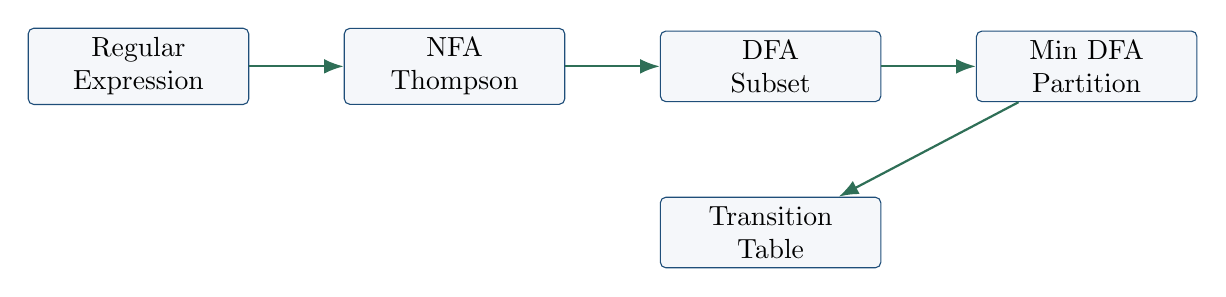
\begin{tikzpicture}[
  node distance=1.2cm,
  box/.style={draw=titleblue, rounded corners=2pt, minimum width=2.8cm, minimum height=0.8cm, align=center, fill=boxgray},
  arr/.style={-{Latex[length=2.5mm]}, thick, draw=softgreen}
]
\node[box] (re) {Regular\\Expression};
\node[box, right=of re] (nfa) {NFA\\Thompson};
\node[box, right=of nfa] (dfa) {DFA\\Subset};
\node[box, right=of dfa] (min) {Min DFA\\Partition};
\node[box, below=of dfa] (table) {Transition\\Table};
\draw[arr] (re) -- (nfa);
\draw[arr] (nfa) -- (dfa);
\draw[arr] (dfa) -- (min);
\draw[arr] (min) -- (table);
\end{tikzpicture}
\end{center}

\subsection{表驱动词法分析}

\begin{itemize}
  \item Lex 的主线是 RE \(\to\) NFA \(\to\) DFA \(\to\) transition table + actions；多个 token 模式可先加新起点，用 \(\epsilon\)-边连接各模式 NFA。 \pg{L2 p49-p54}
  \item 扫描时保存最后一次到达接受态的位置和动作，输入继续前进直到无法转移，再回退到最长接受前缀。 \pg{L2 p55-p59}
  \item DFA 运行时间为 \(O(|X|)\)，每个字符常数时间查表；代价是 subset construction 可能产生 \(2^N\) 个状态。 \pg{L2 p41-p42}
\end{itemize}

\section{CFG、推导与分析树}

\subsection{CFG 基础}

\begin{itemize}
  \item \term{语法分析}{Syntax Analysis/Parser}接收 token 串，判断是否属于语法定义，并构造 parse tree 或 AST。 \pg{L3 p6-p11}
  \item \term{上下文无关文法}{Context-Free Grammar, CFG} 写作 \(G=(V_T,V_N,S,\delta)\)：终结符、非终结符、开始符号、产生式集合。 \pg{L3 p14-p20}
  \item \term{推导}{derivation}是不断用产生式替换非终结符；从开始符号 \(S\) 推出的含终结符/非终结符串叫 \term{句型}{sentential form}，全为终结符时叫 \term{句子}{sentence}。 \pg{L3 p24-p30}
  \item \term{最左推导}{leftmost derivation}每步替换最左非终结符；\term{最右推导}{rightmost derivation}每步替换最右非终结符。 \pg{L3 p29-p30}
\end{itemize}

\subsection{分析树、AST 与二义性}

\begin{itemize}
  \item \term{分析树}{parse tree}隐藏推导顺序，展示产生式层次；无二义性文法中，同一句子的最左/最右推导会得到同一棵分析树。 \pg{L3 p32-p35, L5 p191}
  \item \term{抽象语法树}{Abstract Syntax Tree, AST}是 parse tree 的缩写表示，通常去掉括号、分号等只为语法服务的节点。 \pg{L3 p52}
  \item 若某句子有两棵不同 parse tree，则文法 \term{二义}{ambiguous}。任意 CFG 的二义性判定是不可判定问题。 \pg{L3 p36-p40}
  \item 常见消二义方法是把优先级和结合性写进文法，例如把表达式拆成 \(E,T,F\) 层次，使 \(*\) 比 \(+\) 绑定更紧。 \pg{L3 p40, L4 p35-p50}
\end{itemize}

\subsection{乔姆斯基层级}

\begin{itemize}
  \item Type 0 是 unrestricted grammar；Type 1 是 context-sensitive grammar；Type 2 是 CFG；Type 3 是 regular grammar。 \pg{L3 p43-p49}
  \item 正则文法的产生式形如 \(A\to aB\) 或 \(A\to a\)，表达能力弱于 CFG；程序语言的 token 常由 Type 3 处理，语法结构常由 Type 2 处理。 \pg{L3 p47-p50}
\end{itemize}

\section{自顶向下分析与 LL(1)}

\subsection{递归下降、左递归与左因子}

\begin{itemize}
  \item \term{自顶向下分析}{Top-Down Parsing}从根节点开始构造语法树；\term{递归下降分析}{Recursive-Descent Parsing, RDP}用每个非终结符对应一个函数。 \pg{L4 p5-p12, L6 p61-p62}
  \item 回溯 RDP 会尝试多个候选产生式；\term{预测分析}{Predictive Parsing}要求用有限 lookahead 直接选对产生式，避免回溯。 \pg{L4 p10-p12, L4 p25-p29}
  \item 直接左递归 \(A\to A\alpha|\beta\) 改写为 \(A\to\beta A'\)，\(A'\to\alpha A'|\epsilon\)。多个 \(\alpha_i,\beta_j\) 时写成 \(A\to\beta_1A'|\cdots|\beta_mA'\)，\(A'\to\alpha_1A'|\cdots|\alpha_nA'|\epsilon\)。 \pg{L4 p13-p22}
  \item 公共左因子 \(A\to\alpha\beta_1|\alpha\beta_2\) 改写为 \(A\to\alpha A'\)，\(A'\to\beta_1|\beta_2\)，用于让 lookahead 能区分候选式。 \pg{L4 p27-p29}
\end{itemize}

\subsection{FIRST 与 FOLLOW}

\begin{itemize}
  \item \(FIRST(X)\) 是从符号/符号串 \(X\) 能推导出的首个终结符集合；若 \(X\Rightarrow^*\epsilon\)，则 \(\epsilon\in FIRST(X)\)。 \pg{L4 p30-p38, L4 p46-p48}
  \item 计算 \(FIRST(X_1X_2\cdots X_n)\)：加入 \(FIRST(X_1)-\{\epsilon\}\)，若 \(X_1\) 可空再看 \(X_2\)，依次类推；若全可空，加入 \(\epsilon\)。 \pg{L4 p34-p38}
  \item \(FOLLOW(A)\) 是句型中可能紧跟非终结符 \(A\) 的终结符集合；开始符号的 FOLLOW 包含 \(\$\)。 \pg{L4 p31-p32, L4 p39-p44}
  \item 若 \(B\to\alpha A\beta\)，把 \(FIRST(\beta)-\{\epsilon\}\) 加入 \(FOLLOW(A)\)；若 \(\beta\Rightarrow^*\epsilon\)，把 \(FOLLOW(B)\) 加入 \(FOLLOW(A)\)。 \pg{L4 p39-p44}
\end{itemize}

\subsection{LL(1) 判据与预测分析表}

\begin{itemize}
  \item LL(1) 表示 left-to-right 扫描输入、构造 leftmost derivation、使用 1 个 lookahead。 \pg{L4 p51-p53}
  \item 对任意 \(A\to\alpha|\beta\)，需要 \(FIRST(\alpha)\cap FIRST(\beta)=\varnothing\)；若 \(\epsilon\in FIRST(\alpha)\)，还要 \(FIRST(\beta)\cap FOLLOW(A)=\varnothing\)，反之亦然。 \pg{L4 p51-p52}
  \item 构表规则：对 \(A\to\alpha\)，每个 \(a\in FIRST(\alpha)-\{\epsilon\}\)，填 \(M[A,a]=A\to\alpha\)；若 \(\epsilon\in FIRST(\alpha)\)，对每个 \(b\in FOLLOW(A)\) 填入该产生式。 \pg{L4 p78-p81}
  \item 非递归 LL(1) 算法维护栈和输入缓冲：栈顶是终结符则匹配并弹出；栈顶是非终结符 \(A\) 则查 \(M[A,a]\) 展开；空表项报错。 \pg{L4 p55-p58, L4 p60-p77}
  \item 若一个表项出现多个产生式，说明该文法不是 LL(1)，可能需要消左递归、提左因子，或换更强的 parser。 \pg{L4 p82-p85}
\end{itemize}

\section{自底向上分析与 LR 家族}

\subsection{Shift-Reduce 基础}

\begin{itemize}
  \item \term{自底向上分析}{Bottom-Up Parsing}从输入串逐步归约到开始符号，等价于最右推导的逆过程。 \pg{L5 p4-p7, L5 p60}
  \item Shift-reduce parser 使用栈和输入缓冲，四类动作：shift、reduce、accept、error。 \pg{L5 p6-p8, L5 p37-p44}
  \item \term{句柄}{handle}是在某个最右句型中下一步应被归约的右部；句柄最终会出现在栈顶，因此栈足以支持归约。 \pg{L5 p10-p25}
  \item \term{活前缀}{viable prefix}是不越过最右句柄末端的右句型前缀，是 LR 自动机识别的对象。 \pg{L5 p26-p27}
  \item 冲突包括 shift-reduce conflict 和 reduce-reduce conflict；二义文法常导致冲突，但非二义文法也可能不属于某类 LR。 \pg{L5 p28-p31, L5 p81-p95}
\end{itemize}

\subsection{LR 表与 LR(0) 项}

\begin{itemize}
  \item LR parser 栈中保存状态 \(S_0S_1\cdots S_m\)，ACTION 表按状态和终结符决定移入/归约/接受/错误，GOTO 表按状态和非终结符跳转。 \pg{L5 p34-p44}
  \item \term{增广文法}{augmented grammar}加入 \(S'\to S\)，当归约到该产生式并读到 \(\$\) 时接受。 \pg{L5 p67-p75}
  \item LR(0) \term{项目}{item}是在产生式右部加点，如 \(A\to\alpha\cdot\beta\)，点表示已识别到的位置。 \pg{L5 p64-p66}
  \item \(CLOSURE(I)\)：若 \(A\to\alpha\cdot B\beta\in I\)，对 \(B\to\gamma\) 加入 \(B\to\cdot\gamma\)，直到不再增加。 \pg{L5 p68-p72}
  \item \(GOTO(I,X)\)：把 \(I\) 中点前为 \(X\) 的项目推进一位，再取 closure，得到新状态。 \pg{L5 p72-p77}
  \item 构 LR(0) 表：若状态含 \(A\to\alpha\cdot a\beta\) 且 \(GOTO(I,a)=J\)，则 ACTION 为 shift；若含 \(A\to\alpha\cdot\)，则对所有终结符归约，这也是 LR(0) 容易冲突的原因。 \pg{L5 p74-p84}
\end{itemize}

\subsection{SLR(1)、LR(1)、LALR(1)}

\begin{longtable}{p{0.18\linewidth}p{0.58\linewidth}p{0.16\linewidth}}
\toprule
类别 & 关键思想 & 来源 \\
\midrule
LR(0) & 完成项目立即归约，不看输入符号，能力最弱。 & L5 p80-p95 \\
SLR(1) & 仍用 LR(0) 项集，但只在 lookahead 属于 \(FOLLOW(A)\) 时对 \(A\to\alpha\) 归约。 & L5 p98-p104 \\
LR(1) & 项目带 lookahead，形如 \([A\to\alpha\cdot\beta,a]\)，状态更精细、能力更强。 & L5 p106-p122 \\
LALR(1) & 先构 LR(1)，再合并相同 core 的状态，状态数约等于 SLR，但能力通常接近 LR。 & L5 p124-p137 \\
\bottomrule
\end{longtable}

\begin{itemize}
  \item LR(1) closure：若 \([A\to\alpha\cdot B\beta,a]\in I\)，对每个 \(B\to\gamma\) 和 \(b\in FIRST(\beta a)\)，加入 \([B\to\cdot\gamma,b]\)。 \pg{L5 p109-p121}
  \item LALR 合并同 core 状态，core 是 LR(1) 项去掉 lookahead 后的 LR(0) 项；合并可能引入 reduce-reduce conflict，但不会引入 shift-reduce conflict。 \pg{L5 p126-p131}
  \item 语法能力大致为 \(LR(1) > LALR(1) > SLR(1) > LR(0)\)，实际工具常用 LALR，因为状态数和能力折中较好。 \pg{L5 p137-p139}
  \item LL 与 LR 对比：LL 依据当前非终结符和 lookahead 选择展开；LR 根据已读前缀和 lookahead 决定移入或归约，识别能力通常更强。 \pg{L5 p138}
\end{itemize}

\section{语义分析、SDD 与 SDT}

\subsection{语义分析任务}

\begin{itemize}
  \item \term{语义分析}{Semantic Analysis}是前端最后阶段，检查上下文相关信息，如声明-使用、作用域、类型一致性，是编译器拒绝错误程序的最后前端机会。 \pg{L6 p5-p8}
  \item \term{语法制导定义}{Syntax-Directed Definition, SDD} 是 CFG + 属性 + 语义规则，是翻译的高层说明。 \pg{L6 p13-p16}
  \item \term{语法制导翻译方案}{Syntax-Directed Translation, SDT} 是在产生式右部嵌入 semantic actions 的 CFG，是更接近可执行实现的形式。 \pg{L6 p15-p17}
\end{itemize}

\subsection{属性与依赖}

\begin{itemize}
  \item \term{综合属性}{synthesized attribute}由当前节点的子节点和自身计算，典型例子是表达式值从叶子向上传递。 \pg{L6 p19-p24}
  \item \term{继承属性}{inherited attribute}由父节点、左/右兄弟和自身相关信息计算，常用于把声明类型、环境、偏移等上下文向下或横向传递。 \pg{L6 p22-p25}
  \item 依赖图描述属性求值顺序；必须能拓扑排序，出现环说明属性规则无法直接求值。 \pg{L6 p29-p33, L6 p56}
  \item \term{S-属性定义}{S-attributed definition}只有综合属性，天然适合自底向上 LR 归约时在栈上计算。 \pg{L6 p35, L6 p41-p48}
  \item \term{L-属性定义}{L-attributed definition}允许继承属性，但依赖只能从左到右：右部符号的继承属性可依赖头部继承属性和左侧兄弟属性。 \pg{L6 p36-p37, L6 p49-p73}
\end{itemize}

\subsection{实现与符号表}

\begin{itemize}
  \item S-SDD 转 SDT：把动作放在产生式末尾，归约时执行；栈记录 grammar symbol/state 及属性值。 \pg{L6 p41-p48}
  \item L-SDD 在递归下降中可用函数参数表示 inherited attributes，用返回值表示 synthesized attributes。 \pg{L6 p50-p67}
  \item \term{绑定}{binding}是把标识符使用与定义匹配；\term{作用域}{scope}是定义可见的程序区域。静态作用域由程序文本决定，动态作用域由运行时调用决定。 \pg{L6 p76-p80}
  \item \term{符号表}{symbol table}记录标识符信息，如名字、类型、作用域、存储位置、宽度；多作用域常用 scope stack 管理。 \pg{L6 p81-p93}
  \item \term{类型检查}{type checking}验证类型一致性；静态类型检查在编译期做，动态类型检查在运行时做。 \pg{L6 p94-p99}
\end{itemize}

\section{中间表示、三地址码与回填}

\subsection{IR 与 TAC}

\begin{itemize}
  \item \term{中间表示}{Intermediate Representation, IR}隔离前端和后端，便于支持多语言前端、多目标后端和机器无关优化。 \pg{L7 p4-p11}
  \item \term{三地址码}{Three-Address Code, TAC}右部至多一个运算符，典型形式 \(x=y\;op\;z\)，复杂表达式需拆成临时变量。 \pg{L7 p12-p18}
  \item TAC 地址可以是名字、常量或编译器生成的临时变量；常见指令包括赋值、二元/一元运算、条件跳转、无条件跳转、参数传递、调用、数组读写。 \pg{L7 p14-p17}
  \item \term{四元式}{quadruple}字段为 op、arg1、arg2、result；\term{三元式}{triple}去掉 result，用指令位置引用结果；\term{间接三元式}{indirect triple}用指针表支持代码移动。 \pg{L7 p19-p30}
  \item \term{静态单赋值}{Single Static Assignment, SSA}让每个变量静态上只赋值一次，通过版本号和 \(\phi\) 思想帮助优化判断。 \pg{L7 p31-p33}
\end{itemize}

\subsection{存储布局与数组引用}

\begin{itemize}
  \item 变量布局需要 location 和 width；对齐要求常写成 \(\text{addr}(x)\bmod \text{sizeof}(x.\text{type})=0\)。 \pg{L7 p36-p40}
  \item 二维数组行主序布局中，若 \code{int A[N1][N2]}，元素 \(A[i][j]\) 偏移通常为 \(((i\cdot N_2)+j)\cdot w\)，其中 \(w\) 是元素宽度。 \pg{L7 p48-p52}
  \item 数组翻译常把 base 地址、下标表达式地址、元素宽度和维度大小作为属性传递，最后生成 \(\text{base}[\text{offset}]\) 形式的 TAC。 \pg{L7 p50-p52}
\end{itemize}

\subsection{布尔表达式、控制流与回填}

\begin{itemize}
  \item 布尔表达式可像算术表达式一样计算值，也可直接翻译成跳转；控制语句通常用 true/false label 驱动。 \pg{L7 p54-p58}
  \item \code{if (B) S1 else S2} 的核心是：\(B.true\) 指向 \(S_1\)，\(B.false\) 指向 \(S_2\)，执行完 \(S_1\) 后跳到整体下一条。 \pg{L7 p61-p64}
  \item \term{回填}{backpatching}先生成带空目标的跳转，待标签地址出现后再填入；常用属性有 \(B.truelist\)、\(B.falselist\)、\(S.nextlist\)。 \pg{L7 p64-p70}
  \item 三个基本函数：\(\text{makelist}(i)\) 创建只含指令 \(i\) 的列表；\(\text{merge}(p_1,p_2)\) 合并列表；\(\text{backpatch}(p,i)\) 把列表内跳转目标填为 \(i\)。 \pg{L7 p67-p70}
\end{itemize}

\section{代码优化}

\subsection{基本块与 CFG}

\begin{itemize}
  \item 优化目标可能是执行时间、内存使用、能耗、二进制大小；优化本质是删除、增加、移动或修改代码/数据布局。 \pg{L8 p4-p15}
  \item \term{基本块}{basic block}是直线代码序列：除了第一条指令没有入口标签，除了最后一条没有中途跳出。 \pg{L8 p16-p17}
  \item leader 规则：第一条指令是 leader；任意跳转目标是 leader；任意跳转指令的下一条是 leader。leader 到下一个 leader 前一条构成基本块。 \pg{L8 p20-p22}
  \item \term{控制流图}{Control Flow Graph, CFG} 的节点是基本块，边表示跳转或顺序落入。 \pg{L8 p18-p22}
  \item 局部优化只在一个基本块内做；全局优化跨 CFG，需要证明某性质在所有相关路径上成立，因此必须保守。 \pg{L8 p23, L8 p35-p41}
\end{itemize}

\subsection{DAG 与局部优化}

\begin{itemize}
  \item 基本块 DAG 用节点表示初始值和表达式，可发现公共子表达式、无用赋值和可代数化简的计算。 \pg{L8 p25-p30, L8 p48-p50}
  \item \term{公共子表达式消除}{Common Subexpression Elimination, CSE}：若两次计算操作数和运算符相同且中间值未改变，可复用第一次结果。 \pg{L8 p25-p30}
  \item \term{代数化简}{algebraic identities}：如 \(a*1=a\)、\(a*0=0\)、\(b\&true=b\)。 \pg{L8 p31}
  \item \term{常量折叠}{constant folding}在编译期计算常量表达式；\term{常量传播}{constant propagation}把已知常量代入后续表达式。 \pg{L8 p32-p33}
  \item 若某赋值的变量在基本块出口不 live，则可做 dead code elimination。 \pg{L8 p29-p30}
\end{itemize}

\subsection{全局优化与 LLVM}

\begin{itemize}
  \item 全局常量传播可用 dataflow analysis 在 CFG 上迭代，把人手追踪的“某点变量是否常量”形式化。 \pg{L8 p35-p41}
  \item LLVM 优化以 pass 形式实现：pass 遍历程序某部分收集信息或变换程序。 \pg{L8 p42-p43}
  \item 优化级别：\code{O0} 编译最快、最利于调试；更高优化级通常更快但可能增加编译时间并改变调试体验。 \pg{L8 p44-p45}
\end{itemize}

\section{目标代码生成}

\subsection{后端三大任务}

\begin{itemize}
  \item \term{目标代码生成}{Target Code Generation}把已分析/优化的 IR 转为目标代码，主要考虑代码长度、寄存器使用和机器特性。 \pg{L9 p3-p4}
  \item \term{指令选择}{Instruction Selection}把 IR 映射到目标机器指令；CISC 架构上尤其重要，因为一条复杂指令可能覆盖多个 IR 操作。 \pg{L9 p5, L9 p40-p43}
  \item \term{寄存器分配}{Register Allocation}把变量/临时值放入有限寄存器；不在寄存器中的值需要内存访问，通常更慢。 \pg{L9 p6, L9 p45-p48}
  \item \term{指令调度}{Instruction Scheduling}重排指令以降低延迟、提高流水线/乱序执行效率，同时保持数据依赖正确。 \pg{L9 p44}
\end{itemize}

\subsection{栈式计算机与 MIPS 风格生成}

\begin{itemize}
  \item 栈式计算机没有普通变量/寄存器，操作数压栈，运算从栈顶取数；优化思路是把栈顶保存在 accumulator 中，减少内存访问。 \pg{L9 p7-p11}
  \item MIPS 是 RISC：算术操作用寄存器，内存访问通过 load/store；示例指令包括 \code{lw}、\code{sw}、\code{add}、\code{addiu}。 \pg{L9 p12-p13}
  \item 表达式代码生成函数 \(cgen(e)\) 可约定把结果放入 \code{\$t0}，并保持 \code{\$sp} 与栈内容一致；二元表达式常先算左边并压栈，再算右边并弹出组合。 \pg{L9 p17-p20}
  \item 条件代码生成需要分支指令，如 \code{beq reg1 reg2 label} 和无条件跳转 \code{b label}。 \pg{L9 p20}
\end{itemize}

\subsection{运行时存储与调用约定}

\begin{itemize}
  \item 运行时内存常分 code、global/static、stack、heap；过程每次执行产生一个 \term{活动}{activation}，对应一个 \term{活动记录}{Activation Record, AR}。 \pg{L9 p21-p24}
  \item AR 像栈一样管理：函数入口分配，返回时释放；硬件用 stack pointer \code{\$sp} 指向栈顶。 \pg{L9 p23-p24}
  \item caller-saved registers 由调用者在调用前保存、返回后恢复；callee-saved registers 由被调用者在入口保存、退出前恢复。 \pg{L9 p25-p29}
  \item 调用序列：调用者保存必要寄存器、压入参数、\code{jal label} 跳转并保存返回地址；被调用者建立栈帧，返回时把结果放入 \code{\$v0}，恢复 \code{\$fp}/\code{\$ra}，执行 \code{jr \$ra}。 \pg{L9 p28-p30}
  \item 因为表达式求值会移动 \code{\$sp}，局部变量和参数通常用 frame pointer \code{\$fp} 的固定偏移访问。 \pg{L9 p31-p33}
\end{itemize}

\subsection{面向对象与机器相关优化}

\begin{itemize}
  \item 对象像结构体一样连续布局，成员变量有固定 offset；子类需保持父类成员 offset 不变。 \pg{L9 p34-p39}
  \item 非虚方法可 static dispatch，编译期确定调用目标；虚方法用 dispatch table 动态查找目标。 \pg{L9 p35-p39}
  \item 指令成本可粗略写为 \(1+\text{cost(source-mode)}+\text{cost(destination-mode)}\)，用于比较不同指令选择。 \pg{L9 p42-p43}
  \item \term{寄存器干涉图}{Register Interference Graph, RIG} 中节点是变量，边表示 live range 冲突；无边的变量可放同一寄存器。 \pg{L9 p47}
  \item \(k\)-寄存器分配对应图 \(k\)-着色，是 NP-complete；实际编译器用启发式，多余值通过 \term{溢出}{spilling} 放回内存。 \pg{L9 p48}
  \item \term{窥孔优化}{peephole optimization}在小窗口内改进朴素目标代码，适合删除冗余 load/store、合并简单指令等。 \pg{L9 p49-p50}
\end{itemize}

\section{期末高频题型清单}

\begin{enumerate}
  \item 给 token 规则，写 RE，说明最长匹配和优先级，再把输入串切成 token。 \pg{L1 p33-p39, L2 p55-p62}
  \item 将 RE 转 NFA，再用 \(\epsilon\)-closure 和 move 做 subset construction，最后最小化 DFA。 \pg{L2 p14-p18, L2 p26-p40, L2 p72-p80}
  \item 给 CFG，判断句型/句子，写最左/最右推导，画 parse tree，判断二义性或改写优先级。 \pg{L3 p24-p40, L5 p190-p192}
  \item 消除左递归、提取左因子，计算 FIRST/FOLLOW，构造 LL(1) 表并用栈模拟分析。 \pg{L4 p13-p22, L4 p27-p44, L4 p78-p83}
  \item 构造 LR(0) 项集族、ACTION/GOTO 表，识别 shift-reduce 或 reduce-reduce conflict；说明 SLR/LR(1)/LALR 如何缓解。 \pg{L5 p62-p104, L5 p109-p137, L5 p193-p206}
  \item 给 SDD/SDT，判断 synthesized/inherited、S-attributed/L-attributed，画依赖图或给出属性求值顺序。 \pg{L6 p19-p37, L6 p126-p129}
  \item 把表达式、数组引用、布尔表达式、if/while 翻译成 TAC，使用 truelist/falselist/nextlist 回填。 \pg{L7 p44-p70}
  \item 从 TAC 划分 basic blocks，画 CFG，做 DAG 局部优化、CSE、constant folding/propagation、dead code elimination。 \pg{L8 p16-p33, L8 p48-p50}
  \item 说明目标代码生成中的 instruction selection、calling convention、AR 布局、register allocation、graph coloring 和 spilling。 \pg{L9 p3-p50}
\end{enumerate}

\section{一页速记}

\begin{itemize}
  \item \textbf{词法：}RE 描述 token 模式，FA 实现识别；RE \(\to\) NFA \(\to\) DFA \(\to\) table；最长匹配 + 优先级。 \pg{L1 p22-p36, L2 p49-p62}
  \item \textbf{语法：}CFG 定义结构；LL(1) 自顶向下看 FIRST/FOLLOW；LR 自底向上识别 viable prefix 并用 ACTION/GOTO。 \pg{L3 p14-p20, L4 p51-p83, L5 p34-p44}
  \item \textbf{语义：}SDD 是规则，SDT 是嵌入动作；S-属性适合 LR，L-属性适合 LL/RDP 或转化实现。 \pg{L6 p13-p17, L6 p35-p73}
  \item \textbf{IR：}TAC 一条指令最多一个运算；quadruple 易重排结果，triple 省 result 但移动麻烦，indirect triple 用指针表缓解。 \pg{L7 p12-p30}
  \item \textbf{优化：}先划分 basic block 和 CFG；局部用 DAG，全球用 dataflow；任何优化都必须保持语义。 \pg{L8 p16-p41}
  \item \textbf{后端：}目标代码生成三件事是指令选择、寄存器分配、指令调度；函数调用靠 AR、\code{\$sp}/\code{\$fp}/\code{\$ra} 和 caller/callee saved 约定。 \pg{L9 p3-p30}
\end{itemize}

\end{document}
